%%%%%%%%%%%%%%%%%%%%%%%%%%%%%%%%%%%%%%%%%%%%%%%%%%%%%%%%%%%%%%%%%%%%%%%%%%%%%%%
%
% Purpose:  Detailed part of Product Spec for the time model
%
% 
%
%%%%%%%%%%%%%%%%%%%%%%%%%%%%%%%%%%%%%%%%%%%%%%%%%%%%%%%%%%%%%%%%%%%%%%%%%%%%%%%


\subsection{Functional Design} \label{ref:FunctionalDesign}
See the \href{file:refman.pdf}{Reference Manual} 
\cite{timebib:ReferenceManual} for a summary of member data and member methods 
for all classes.  This section describes the functional operation of the 
methods in each class.

Objects are presented in alphabetical order.
Methods are presented in alphabetical order within the object in
which they are located.  
Methods that are inherited from a parent class
are described in that parent class.

{\begin{enumerate}

\classitem{JeodBaseTime}\label{ref:Time} Base-class

{\begin{enumerate}

\funcitem{add\_type\_initialize}
\label{ref:addtypeinitialize}Specific to each time-type.  If not
specified for a time-type, causes a termination.  This function is
specified in classes \reftext{TimeUDE}{ref:TimeUDE} and 
\reftext{TimeStandard}{ref:TimeStandard}, but
not in \textit{TimeDyn}.

\funcitem{add\_type\_update} 
Recursively adds elements to the update tree. If the
``parent'' to a time-type is defined but not
already in the tree, it calls itself on the
``parent'' then returns to adding the
``child'' type. If the
``parent'' is not defined it searches for a
suitable ``parent'' from the types already in
the tree.  If that search is successful, it adds the
``child'' to the tree, otherwise it returns
without change.

\funcitem{initialize\_from\_parent}
Specific to each time-type.  If not specified for a time-type, this method 
causes a
termination.  This method is specified in classes 
\reftext{TimeUDE}{ref:TimeUDE} and \reftext{TimeStandard}{ref:TimeStandard}, 
but not in \textit{TimeDyn}.

\funcitem{initialize\_initializer\_time }
Pure-virtual function.

\funcitem{must\_be\_singleton}
Returns true by default, indicating that there can be only one type of a
particular object.

\funcitem{set\_time\_by\_days}
Takes an input value, and sets the value \textit{days }to that value,
and the value \textit{seconds} to 86,400 times that value.

\funcitem{set\_time\_by\_seconds}
Takes an input value, and sets the value \textit{seconds} to that value,
and the value \textit{days} to 1/86,400 of that value.

\funcitem{update}
Calls the appropriate converter to update the time from its parent.

\end{enumerate}}


\classitem{TimeConverter} \label{ref:TimeConverter} Base-class

This is the abstract class that describes the basic structure needed by all
converters.  The different subclasses each describe the conversion process 
between a
specified pair of time-types.  Only a small subset of potential
pairings are included in the release of \JEODid, although that small
subset does provide complete coverage of all the clock representations.



\begin{table}[h]
   \caption{Availability of Converter Functions} 
\vspace{0.25in}
\ \ \ \ This table shows which converter functions are available in the 
standard release.
   
\ \ \ \ 1 -- available for initialization only

\ \ \ \ 2 -- available for updates only
         
\ \ \ \ 3 -- available for initialization and updates.
         
\ \ \ \ * -- by inheritance.
\vspace{0.25in}
         
         
   \centering
   \label{tab:ConverterFunctions} 
      \begin{tabular}{||l|l|l|l|l|l|l|l|l|l|l|l||} \hline
   \ \ \ \ \ \ \ To: &Dyn &GMST &GPS &MET &STD &TAI &TDB &TT &UDE &UT1 &UTC\\
From: &~ &~ &~ &~ &~ &~ &~ &~ &~ &~ &~\\ \hline
Dyn &~ &~ &~ & 3* &~ & 2 & 2 & 3 &~ &~\\\hline
GMST &~ &~ &~ &~ &~ &~ &~ &~ &~ &~ &~\\\hline
GPS &~ &~ &~ &~ &~ & 3 &~ &~ &~ &~ &~\\\hline
MET &~ &~ &~ &~ & 3* &~ &~ &~ &~ &~ &~\\\hline
STD &~ &~ &~ & 3* &~ &~ &~ &~ & 3 &~ &~\\\hline
TAI &~ &~ & 3 &~ &~ &~ & 3 & 3 &~ & 3 & 3 \\\hline
TDB &~ &~ &~ &~ & 3 &~ &~ &~ &~ &~\\\hline
TT &~ &~ &~ &~ &~ & 3 &~ &~ &~ &~ &~\\\hline
UDE &~ &~ &~ &~ & 3 &~ &~ &~ &~ &~ &~\\\hline
UT2 &~ & 3 &~ &~ &~ & 3 &~ &~ &~ &~ &~\\\hline
UTC &~ &~ &~ &~ &~ & 1 &~ &~ &~ &~ &~\\\hline

   \end{tabular}
   
   
   
   
\end{table}

{\begin{enumerate}

\funcitem{can\_convert}
Specific to each converter type (not to each instance). Extended classes may  
combine these options using bitwise "OR" when assigning in the constructor.

To check whether the converter can accept any combination of directions, the 
user may utilize the can\_convert() function

NO\_DIRECTION : null, no direction specified

A\_TO\_B\_INIT : able to initialize the second time from the first

B\_TO\_A\_INIT : able to initialize the first time from the second

A\_TO\_B\_UPDATE : able to update the second time from the first

B\_TO\_A\_UPDATE : able to update the first time from the second

A\_TO\_B : always able to convert the second time from the first

B\_TO\_A : always able to convert the first time from the second

ANY\_DIRECTION : always able to convert the two times


\funcitem{initialize}\label{ref:TimeConverterinitialize} 
Pure-virtual function.

Each subclass must define its own version of this function, but they
all have some similarities.

Each time converter has the potential to contain two functions, a
converter from \textit{aaa} to \textit{bbb}, and a converter from
\textit{bbb} to \textit{aaa}.

The initialize function receives 3 arguments -- a pointer to a
time-type labeled as \textit{parent, }a pointer to a time-type labeled
as \textit{child, }and an integer  $\pm 1$ that identifies whether
\textit{aaa }is associated with \textit{parent, }or \textit{child.}

The converter is initialized for conversion either from \textit{aaa} to
\textit{bbb }or for conversion from \textit{bbb} to\textit{ aaa.
}However, the initialization of the converter then allows the
conversion in both directions, if that functionality exists.  This is
best seen in an example:

\begin{quotation}
Suppose that when building the tree, the TimeManager identifies that
time-type \textit{xxx} is calculated from time-type \textit{yyy.  }It
identifies that a time-converter, \textit{TimeConverter\_xxx\_yyy} has
been registered for this type of conversion, and that this converter
has not been initialized.  It calls
\textit{TimeConverter\_xxx\_yyy:: initialize(yyy\_ptr, xxx\_ptr, -1)}
because \textit{yyy} is the \textit{parent} and \textit{xxx} the
\textit{child} for the intended conversion.  If the converter is not
able to convert from \textit{yyy} to \textit{xxx}, the tree that has
been defined is invalid, and the code will terminate here.  This
initialization will then also allow conversions from \textit{xxx }to
\textit{yyy} if the \textit{convert\_a\_to\_b} function is defined.
\end{quotation}

\normalsize
The \textit{verify\_setup} function is called with the same arguments. 
In order for the verification to proceed, one of the two types --
\textit{child} or \textit{parent} -- must be already initialized.  This
type is called the\textit{ master.  }In most cases, the \textit{parent}
type becomes the \textit{master} type for the verification, but there
are exceptions.  See
\reftext{Time\_Converter\_dyn\_tai::initialize}{ref:TimeConverterdyntaiinitialize} 
for discussion.  

Next, the \textit{parent\_ptr} and \textit{child\_ptr} are cast into
their respective time-types, and a check made that they are of the
time-type that they are supposed to be.

Finally, the initial value \textit{a\_to\_b\_offset } may be calculated,
which can (in some cases) be used in the \textit{convert\_a\_to\_b} and
\textit{convert\_b\_to\_a} functions.  In some converters, this initial
value remains unchanged throughout the simulation.

\funcitem{verify\_setup}
This function is used by each of the \textit{TimeConverter\_xxx\_yyy} classes 
to verify that sufficient data exists to allow the converter to be
initialized.  The following criteria must all be met or the code will
terminate:

\begin{enumerate}
\item Of the two time-types associated with the converter, one
(identified as the \textit{master }in this function) must already be
initialized.
\item Both time-types must have known memory addresses.
\item {\itshape
\textup{A direction} (1 or -1, indicating xxx is master or yyy is master
respectively) \textup{must have been }\textup{defined.  }}
\end{enumerate}

\funcitem{verify\_table\_lookup\_ends}
Has no functionality at this level, simply returns to the calling routine.

\end{enumerate}}

\classitem{TimeConverter\_Dyn\_TAI}
\textref{TimeConverter}{ref:TimeConverter}


{\begin{enumerate}
\funcitem{initialize}\label{ref:TimeConverterdyntaiinitialize}
See the base-class version of 
\textref{initialize}{ref:TimeConverterinitialize} for overall description.

Because \textit{TAI} has an absolute reference, and \textit{dyn-time}
does not, the initial value of \textit{TAI} must be known to initialize
the offset between them.  Therefore, the \textit{master} type must be
\textit{TAI} independent of which is the \textit{parent}.  The
\textit{initialize} function could be called with the intention of
confirming \textit{TAI} to \textit{Dyn} conversion capability or
\textit{Dyn} to \textit{TAI} conversion capability, but either way, the
\textit{master} must be \textit{TAI}. Calling \textit{verify\_setup}
with\textit{ master = Dyn }would fail to provide the protection that
this function is intended to provide.

Once initialized, the offset between \textit{Dyn} and \textit{TAI} is
constant throughout the simulation.

\funcitem{can\_convert}
valid\_directions:
A\_TO\_B\_UPDATE

For runtime only.  The offset between \textit{time\_dyn} and
\textit{time\_tai }is constant throughout a simulation. 
Knowledge of this
offset and of the value \textit{dyn\_time} allows for a trivial calculation of
\textit{time\_tai}.
\end{enumerate}} 



\classitem{TimeConverter\_Dyn\_TDB}
\textref{TimeConverter}{ref:TimeConverter}


{\begin{enumerate}
\funcitem{initialize}\label{ref:TimeConverterdyntdbinitialize}
See the base-class version of 
\textref{initialize}{ref:TimeConverterinitialize} for overall description.

Because \textit{TDB} has an absolute reference, and \textit{dyn-time}
does not, the initial value of \textit{TDB} must be known to initialize
the offset between them.  Therefore, the \textit{master} type must be
\textit{TDB}independent of which is the \textit{parent}.  The
\textit{initialize} function could be called with the intention of
confirming \textit{TDB} to \textit{Dyn} conversion capability or
\textit{Dyn} to \textit{TDB} conversion capability, but either way, the
\textit{master} must be \textit{TDB}. Calling \textit{verify\_setup}
with\textit{ master = Dyn }would fail to provide the protection that
this function is intended to provide.

Once initialized, the offset between \textit{Dyn} and \textit{TDB} is
constant throughout the simulation.

\funcitem{can\_convert}
valid\_directions:
A\_TO\_B

The offset between \textit{time\_dyn} and
\textit{time\_tdb} is constant throughout a simulation. 
Knowledge of this
offset and of the value \textit{dyn\_time} allows for a trivial calculation of
\textit{time\_tdb}.




\end{enumerate}}


\classitem{TimeConverter\_Dyn\_UDE}
  \textref{TimeConverter}{ref:TimeConverter}

There can be multiple instances of this class.

{\begin{enumerate}
\funcitem{initialize}
See the base-class version of 
\textref{initialize}{ref:TimeConverterinitialize} for overall description.

This function is similar to the \textref{Dynamic Time to TAI initializer}
{ref:TimeConverterdyntaiinitialize},
in that the UDE time may have a defined initial value known only to
TimeUDE.  The \textit{master} type must be \textit{UDE, }even though
\textit{Dyn} is always going to be the \textit{parent}.  The
\textit{initialize} function could be called with the intention of
confirming \textit{Dyn} to \textit{UDE} conversion capability, but the
\textit{master} must still be \textit{UDE.  }Calling
\textit{verify\_setup} with\textit{ master = Dyn }would fail to provide
the protection that this function is intended to provide.

Once initialized, the offset between \textit{Dyn} and \textit{UDE} is
typically constant throughout the simulation.  The exception to this is
the case of a \textit{MET }(subclass of \textit{UDE}), which allows
for hold-points in the simulation.  In this case, the offset will be
adjusted accordingly during the simulation.

\funcitem{can\_convert}
valid\_directions:
A\_TO\_B

The offset between \textit{time\_dyn }and
\textit{time\_ude }is well known throughout a simulation. 
\textit{time\_ude} can easily be calculated with knowledge of this
offset and of the value \textit{dyn\_time.}

\end{enumerate}}

\classitem{TimeConverter\_STD\_UDE}
  \textref{TimeConverter}{ref:TimeConverter}

There can be multiple instances of this class.

{\begin{enumerate}
\funcitem{can\_convert}
valid\_directions:
ANY\_DIRECTION

For run-time and initialization.

\funcitem{initialize}
See the base-class \textref{initialize}{ref:TimeConverterinitialize} method 
for overall description.

\funcitem{reset\_a\_to\_b\_offset}
In the event that a hold was placed on the UDE time, the offset between
the two times will change.  This function simply recalculates the
offset by differencing the two times once the hold has been removed.
\end{enumerate}}



\classitem{TimeConverter\_TAI\_GPS}
  \textref{TimeConverter}{ref:TimeConverter}

The difference between the Truncated Julian Time values of \textit{GPS}
epoch time and \textit{TAI} epoch time is taken (these default to
midnight UTC on January 5/6, 1980, and J2000 respectively).  This gives
a difference in days, which is used to calculate the offset.  The
offset remains constant though the simulation.

{\begin{enumerate}
\funcitem{can\_convert}
valid\_directions:
ANY\_DIRECTION

For run-time and initialization. 

\funcitem{initialize}
See the base-class \textref{initialize}{ref:TimeConverterinitialize} method 
for overall description.


\end{enumerate}}

\classitem{TimeConverter\_TAI\_TDB}
  \textref{TimeConverter}{ref:TimeConverter}

The offset between these two times can be calculated from an analytic
function to a very high degree of precision each time it is needed.  It
is not given an initial value.

{\begin{enumerate}
\funcitem{can\_convert}
valid\_directions:
ANY\_DIRECTION

For run-time and initialization. Converter is straightforward, TDB is an 
analytic function of TAI. A generalized version of the code is provided below.
\begin{verbatim}
void TimeConverter_XXX_YYY::convert_a_to_b (void)
{
	set_a_to_b_offset();
	yyy_ptr->set_time_by_seconds (xxx_ptr->seconds + a_to_b_offset - 
				      a_to_b_offset_epoch);
	return;
}

void TimeConverter_XXX_YYY::convert_b_to_a (void)
{
	xxx_ptr->set_time_by_seconds(prev_xxx_seconds + (yyy_ptr->seconds - prev_yyy_seconds));
	while(true) {
		nSteps++;
		nIter++;
		set_a_to_b_offset();
		double dXXX = (yyy_ptr->seconds - xxx_ptr->seconds)
			    - (a_to_b_offse - a_to_b_offset_epoch);
		xxx_ptr->set_time_by_seconds(xxx_ptr->seconds + dXXX);
		
		if (nSteps > 5 || std::abs(dXXX/xxx_ptr->seconds) < std::pow(10,-15)) {
			break;
			prev_yyy_seconds = yyy_ptr->seconds;
			prev_xxx_seconds = xxx_ptr->seconds;
		}
	}
}
\end{verbatim}

\funcitem{initialize}
See the base-class \textref{initialize}{ref:TimeConverterinitialize} method 
for overall description.


\end{enumerate}}

\classitem{TimeConverter\_TAI\_TT}
  \textref{TimeConverter}{ref:TimeConverter}

TT is derived from the old ephemeris time which, at the time of its
definition epoch, happened to have an offset of 32.184 seconds, or
0.0003725 days.  This offset is constant.

{\begin{enumerate}
\funcitem{can\_convert}
valid\_directions:
ANY\_DIRECTION

\funcitem{initialize}
See the base-class \textref{initialize}{ref:TimeConverterinitialize} method 
for overall description.

\end{enumerate}}

\classitem{TimeConverter\_TAI\_UT1}
  \textref{TimeConverter}{ref:TimeConverter}


The techniques used in the TAI to UT1 converter are similar to those in 
\textref{Time\_Converter\_TAI\_UTC}{ref:TimeConverterTAIUTC}.  
The main difference is
that both UT1 and TAI are continuous, and the offset between them is
calculated by an interpolation between the boundary points of the time
interval in the \textit{tai\_to\_ut1 }table.  This avoids the problem
of handling discontinuities that are discussed in the 
\textref{TAI to UTC converter}{ref:TimeConverterTAIUTC}, but introduces another
concern over interpretation of data.

The lookup times in the TAI\_to\_UT1 tables can be interpreted as being
either TAI or UT1, but that interpretation must be consistent.  The
arbitrary interpretation is permitted because they differ by so little,
and that difference changes so slowly.  That difference is typically
$TAI-UT1 \sim 30 \; s$,
it changes by  $O(10^{-3}) \; s \cdot day^{-1}$ and is calculated out to 
$O(10^{-4}) \; s$.  Making a wrong interpretation introduces an error that
is at most the product of the gradient with the maximum difference,
equating to  $O(10^{-7})\; s$, which is well within the precision of the
tables themselves.  Because UT1 is typically updated from TAI, it is
assumed that these tables represent the lookup times as a TAI
representation.

Nevertheless, if the interpretation is inconsistent, it would be
possible to use TAI to find UT1, then use that value to convert back to
TAI, ad infinitum, progressing time artificially.  A particular example
is the situation in which TAI is initialized based on a UT1 time, then
UT1 updated from TAI; because UT1 is calculated from TAI there would
first be a UT1-based lookup to generate TAI, then a runtime TAI-based
lookup to generate UT1.  Not accounting for the difference would result
in the simulation starting at a time $O(10^{-7}) \; s$ different to when it
was intended to start.  This leads to a difference in the way the two 
converters
function.



{\begin{enumerate}
\funcitem{can\_convert}
valid\_directions:
ANY\_DIRECTION

Since UT1 is calculated from TAI by the linear interpolation of points
in the tables, we have:

\begin{equation}
\mathit{UT1}=\mathit{TAI}+\left(\mathit{offset}_{\mathit{prev}}+(\mathit{TAI}-\
mathit{when}_{\mathit{prev}})\mathit{grad}\right)
\end{equation}
where 

$\mathit{offset}_{prev}$ is the most recent entry in the
TAI-to-UT1 conversion table, giving the value UT1 - TAI,

${when}_{prev}$ is the TAI time corresponding to 
$\mathit{offset}_{prev}$,

and
\begin{equation*}
grad=\frac{{\mathit{offset}_{next}-\mathit{offset}_{prev}}}{{when}_{next}-{when
}_{prev}}
\end{equation*}

While it is not appropriate to use the same linear interpolation to
obtain TAI, this expression can be rearranged to give a comparable

\begin{equation*}
\mathit{TAI}=\mathit{UT1}-
\left(\frac{\mathit{offset}_{\mathit{prev}}+
\left(\mathit{UT1}-\mathit{when}_{\mathit{prev}}\right)\mathit{grad}}
{1+\mathit{grad}}\right)
\end{equation*}

(Note that  $\mathit{when}_{\mathit{prev}}$ is still TAI time, with a
corresponding UT1 time of 
$(\mathit{when}_{\mathit{prev}}+\mathit{offset}_{\mathit{prev}})$)

In most situations, this is sufficient, but a problem occurs when the
gradient calculated based on the UT1 time input is different to that
for the TAI time output, i.e. when the TAI and UT1 times are in
different {\textquotedblleft}boxes{\textquotedblright} in the tables. 
The gradient in the above equation should be associated with the TAI
time, but it is first identified from the UT1 time.  To circumvent this
problem, the value that the UT1 time is compared against is not the 
interval boundary
(known in TAI time), but the sum of the interval boundary and the
offset at that boundary (UT1 time at the boundary).  Because UT1 is
continuous at the boundaries of each
{\textquotedblleft}box{\textquotedblright}, this eliminates the
inconsistency.

\funcitem{initialize}
See the base-class \textref{initialize}{ref:TimeConverterinitialize} method 
for overall description.




\funcitem{initialize\_tai\_to\_ut1}
This function is used to initialize the converter from TAI to UT1, and
set up the tables for future updates.

It has similarities to 
\textref{initialize\_leap\_seconds}{ref:initializeleapseconds} in
setting up the table.  Unlike the TAI to UTC conversion function, which
has discontinuities, the TAI to UT1 conversion is a smooth function and
requires that the previous and next data values be considered, and the
slope between them calculated in order to interpolate between points in
the tables.

\funcitem{verify\_table\_lookup\_ends}
This function is necessary for those converter classes that utilize
lookup tables.  If a simulation time passes beyond the domain of a
lookup table, the value of the offset is set to be the last known
value, and a flag is set to indicate that further (time-consuming)
calls to the table are not necessary.  This flag must be reset if the
simulation reverses time; this function resets that flag.

\end{enumerate}}

\classitem{TimeConverter\_TAI\_UTC}\label{ref:TimeConverterTAIUTC}
  \textref{TimeConverter}{ref:TimeConverter}

The conversion between TAI and UTC is based on lookup
tables that provide the offset as a function of time.  The times in
those tables are UTC times, showing when leap seconds were
introduced.  In the cases that the offset value is artificially forced
to remain constant (\textit{true\_utc = false,} for comparison to
JEOD 1.x.x) or the current time is outside the range of the data table,
the offset value is constant and the conversion trivial in either
direction.  It is recommended that TAI be updated from
 Dynamic Time, and UTC updated from TAI; this makes
TAI smooth and UTC discontinuous, with repetition at
leap seconds (hence, there is no Dynamic Time to UTC converter
provided).

{\begin{enumerate}
\funcitem{can\_convert}
valid\_directions:
A\_TO\_B and B\_TO\_A\_INIT

For converting from TAI to UTC, UTC is first calculated from the
previously known offset.  This value is then used for comparing against
the boundaries.  If the time has passed through a leap second value,
the UTC representation is recalculated based on the corrected number of
leap seconds, and tested again.

The conversion from TAI to UTC has issues at leap seconds. 
Because UTC is calculated from the previously known offset, it will
pass through midnight before the new offset is identified.  A typical
sequence of UTC times, updated every 0.2 seconds may be
(day:hour:minute:second)  

{\itshape
[0:23:59:59.8 ,  0:23:59:60.0 = 1:00:00:00.0 ={\textgreater}
1:00:00:(-1.0) = 0:23:59:59.0 , 0:23:59:59.2 etc. ] }

Triggering the leap second at midnight causes UTC to momentarily progress one
day, then back up again into the
previous day, which is not a realistic representation.  Of course, the
alternative of triggering it at midnight + 1 second is worse since it
causes UTC to start the next day 1 second early.  This is the best
solution available.

For converting UTC to TAI at initialization, the UTC value is
compared to the recorded boundaries of the current calibration interval
(\textit{prev\_when} and \textit{next\_when}).  If it is outside the
boundary, then the values of the boundaries and the value of the offset
between UTC and TAI are adjusted accordingly.  There
is also verification that the current time has not passed the end of
the calibrated data.  

The conversion function from UTC to TAI is
fundamentally flawed at the times where leap seconds are added;
UTC normally ticks 23:59:59 to 23:59:60 = 00:00:00, except at
leap seconds when it ticks 23:59:59 to 23:59:60 to 00:00:00.  However,
the Julian representation reads 23:59:60 and 00:00:00 as being the same
time.  The result is that the UTC value in the new day ticks
from 0 to 1 second, jumps back to 0, and restarts, causing there to be
two TAI values for any given UTC time in that
interval.  The code does not have the capacity to uniquely represent times 
in the interval  $t\in $\textit{[23:59:60, 23:59:61)} UTC. 
The problem really only shows itself at initialization (unless the user
chooses to declare this converter valid at runtime).  
Even though 23:59:60.5  UTC may exist in reality,
the code will interpret that value as being 1 second later, 00:00:00.5.
 Users should therefore avoid initializing a simulation using a
UTC value during a leap second interval.


\funcitem{initialize}
See the base-class \textref{initialize}{ref:TimeConverterinitialize} method 
for overall description.

\funcitem{initialize\_leap\_seconds}\label{ref:initializeleapseconds}
This function is used to initialize the UTC to TAI converter, in
conjunction with \textit{initialize} above.

The conversion between TAI and UTC utilizes a lookup table, which
tabulates when leap seconds were added.  The times used in the table
are in a UTC representation, and the result is the difference between
TAI and UTC.  

Initially, a test is made whether the current UTC time is covered by the
tables.  If not, the end-value from the table is used; there is no attempt made
to extrapolate the occurence of leap seconds either into the future, or before
1972.

In the event that the UTC time is not within the table range and never will 
be, a flag
\textit{off\_table\_end} is set to true; this has the effect of
removing the lookup from the subsequent process.  

If the current UTC time is within the boundaries of the table, then the
number of leap seconds appropriate for that time is identified and
recorded as (negative) \textit{a\_to\_b\_offset.}

\funcitem{verify\_table\_lookup\_ends}
This function is necessary for those converter classes that utilize
lookup tables.  If a simulation time passes beyond the domain of a
lookup table, the value of the offset is set to be the last known
value, and a flag is set to indicate that further (time-consuming)
calls to the table are not necessary.  This flag must be reset if the
simulation reverses time; this function resets that flag.

\end{enumerate}}


\classitem{TimeConverter\_UT1\_GMST}
  \textref{TimeConverter}{ref:TimeConverter}


{\begin{enumerate}
\funcitem{can\_convert}
valid\_directions:
A\_TO\_B

For run-time and initialization, this algorithm is based on the
Astronomical Almanac \cite{timebib:AstronomicalAlmanac}, 
with some simplification to account for our
ability to count in days since J2000.  The algorithm in the
Astronomical Almanac uses days since noon on January 1, 2000
\textit{UT1}.  We carry days since J2000 (noon of January 1, 2000,
\textit{TT}), which is slightly different.  To reconcile this
difference, we first subtract off the difference between the two
values, which corresponds to a little over a minute, or 0.00738762
days.

\begin{equation*}
d=days_{UT1}-0.000738762
\end{equation*}

(where  $days_{UT1}$ is days of \textit{UT1} time since
J2000).

Then, the Astronomical Almanac algorithm can be expressed as:
\begin{equation}
\mathit{days}_{\mathit{GMST}}=0.7790572733+1.002737909350795d+8.0775E-16d^{2}-1.5E-24d^{3}
\end{equation}
and this value used to set \textit{GMST} values by days.

\funcitem{initialize}
See the base-class version of 
\textref{initialize}{ref:TimeConverterinitialize} for overall description.


\end{enumerate}}

\classitem{TimeDyn}\label{ref:TimeDyn}
  \textref{JeodBaseTime}{ref:Time}


{\begin{enumerate}
\funcitem{initialize\_initializer\_time}
Initializes the simulation only if there are no Standard Times present
in the simulation.

\funcitem{update}
Updates the Dynamic Time value directly from the Simulator Time, using
$t_{d}=\alpha t_{s}+\delta $, where:


\begin{itemize}
\item  $t_{d}$ represents Dynamic Time (seconds)
\item  $t_{s}$ represents the Simulator Time (seconds)
\item  $\alpha $ represents the scale factor between the rate at which
Dynamic Time advances, and the rate at which the Simulator Time/counter
advances.  This is user-defined, and defaults to 1.0.
\item  $\delta $ represents the offset between the Simulator Time and
the Dynamic Time.  This value is auto-generated, and defaults to 0.0. 
See \textref{update\_offset}{ref:updateoffset} for description of this value.
\end{itemize}

\funcitem{update\_offset}\label{ref:updateoffset}
The Dynamic Time advances linearly with the
Simulator Time, at some user-defined rate (default = 1.0), and with
some \textit{offset} value that represents the value of Dynamic Time
when Simulator Time = 0.0.  At the start of all simulations, both
Dynamic Time and Simulator Time are initialized at 0.0, and the offset
is therefore also 0.0.  However, if the rate at which time advances
changes mid-simulation, the offset must be recalculated.

Dynamic Time contains some public and private elements relating to the rate
and direction in which time advances.  The public element,
\textit{scale\_factor}, can be changed in the input file but is not
used directly anywhere in the code.  Conversely, the private
element,\textit{ ref\_scale,} is actually used in updating Dynamic Time, and
can only be changed here.

Only if the private and public elements disagree has a change been made
to the public values.  If the public values have changed, the private
values must be updated, and the offset between Simulator Time and Dynamic Time
recalculated.  

In the following illustration, Dynamic Time and Simulator Time advance
together.  \textit{Offset} retains its default value of 0.0.  At some
point (A in figure) Dynamic Time is slowed for enhanced resolution, and
\textit{offset} is calculated (to a).  As long as the rate remains
constant, \textit{offset} will also remain constant.  At some time
later (B in figure), the rate of Dynamic Time with respect to simulator
time is reverted to its original value.  At this point, \textit{offset} does
not revert back to 0.0; instead, it is recalculated to give the value
represented by b in the figure.

This function serves dual purpose.  First, it tests whether the rate (or
\textit{scale\_factor}) has changed, and recalculates \textit{offset}
only if it has.  Secondly, it returns a true/false flag indicating the
result of that test; this flag can then be used in other routines as
necessary without further testing (e.g. integration algorithms that
retain a history will have to be reset every time
\textit{scale\_factor} is changed).

\begin{figure}[htp]
\begin{center}
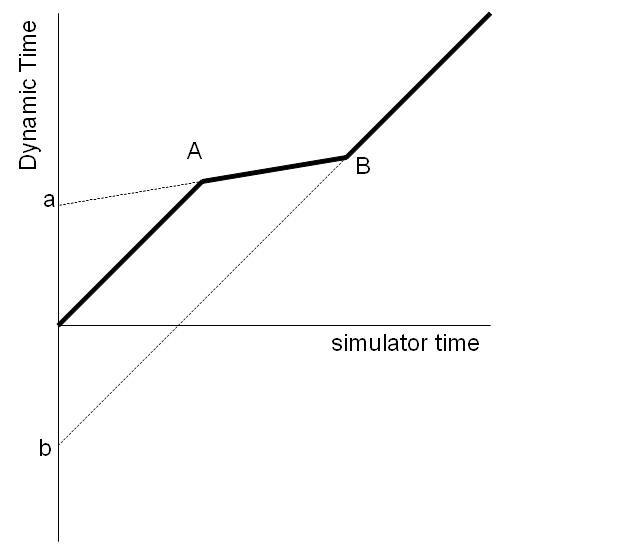
\includegraphics[width=3.2736in,height=2.85in]{figures/Timedyntime.jpg}
\caption{Illustration of how Dynamic Time can vary with Simulator Time, 
and the resulting effect on the offset between them.}
\end{center}
\end{figure}

\end{enumerate}}


\classitem{TimeEnum} Base-class

This class contains no methods, just an enumeration.

\begin{enumerate}
\item Julian.
\item Modified Julian.
\item Truncated Julian.
\item Calendar.
\item Clock.
\item Days since epoch.
\item Seconds since epoch.
\end{enumerate}



\classitem{TimeGMST}
  \textref{TimeStandard}{ref:TimeStandard}

{\begin{enumerate}
\funcitem{set\_time\_by\_trunc\_julian}
Even though GMST is technically a Standard Time, Truncated Julian Time
has no meaningful interpretation, since it is based on a synodic clock.
 This function overrides the one inherited from \textref{TimeStandard}{ref:TimeStandard}
by causing a termination if anything attempts to use Truncated Julian
Time in GMST.

\funcitem{calculate\_calendar\_values}
Even though GMST is technically a Standard Time, the calendar that is an
element of Standard Time  has no meaningful interpretation, since it is
based on a synodic clock.  This function overrides the one inherited
from \textref{TimeStandard}{ref:TimeStandard} by causing a termination if anything
attempts to use a calendar in GMST.

\end{enumerate}}



\classitem{TimeGPS}
 \textref{TimeStandard}{ref:TimeStandard}


GPS time is somewhat unusual.  It fits the definition of a Standard Time
(it is well defined), but does not maintain the same counters as a
typical clock.  Instead of days, months, etc., it uses weeks and
seconds of week since epoch (there is also a \textit{rollover} count,
used because the number of weeks since epoch has now exceeded its
counting capacity of 1,024 weeks).

{\begin{enumerate}
\funcitem{calculate\_calendar\_values}
The conventional concept of calendar makes no sense in the GPS
timekeeping system.  All GPS values are maintained all of the time, and
any call to this function will produce a code termination.

\funcitem{set\_time\_by\_days}
Converts number of days since epoch into weeks and seconds of week since
epoch.

\funcitem{set\_time\_by\_seconds}
Converts number of seconds since epoch into weeks and seconds of week
since epoch.

\funcitem{set\_time\_by\_trunc\_julian}
The epoch is hard-coded in Truncated Julian Time, so it is trivial to
convert any given Truncated Julian Time and change that into days or
seconds since epoch.

\end{enumerate}}
\classitem{TimeManager} Base-class


{\begin{enumerate}
\funcitem{get\_converter\_ptr}
As each converter is registered, it is stored in a vector and is assigned an
index value equal to its position within that vector.  
This function returns a pointer to any particular
converter given its index in that vector.

\funcitem{get\_time\_change\_flag}
The \textit{time-change-flag} is triggered if the Dynamic Time scale
factor is changed (see \textref{update\_offset}{ref:updateoffset}).  
This function simply returns
the boolean indicating whether the scale factor changed since the last
time step.

\funcitem{get\_time\_ptr}
There are two instances of this function, one takes a name, and the
other takes an index.  When a time representation is registered with
the Time Manager, a pointer to it is stored in a vector.  All time
representations also have a unique name.  This function returns the
pointer to the time representation using either value as a reference.

\funcitem{initialize}
Registers and initializes the Dynamic Time.

Counts the number of time-types registered from the S\_define.

Calls \textit{TimeManagerInit::initialize\_manager}.

Runs an update on all time-types at Dynamic Time = 0.0.

\funcitem{register\_converter}
Called from the S\_define level, this function simply appends a pointer to
each converter onto the \textit{time\_converters\_ptrs}
vector.  This function is used when the converter is between two
specific time representations (e.g. TAI and UTC).

\funcitem{register\_generic\_converter}
Called from the S\_define level, this function simply appends a pointer to
each converter onto the \textit{time\_converters\_ptrs}
vector.  This function is used when one or both of the two time
representations is not a Standard Time (i.e. is a UDE or MET).  This
function requires naming the non-Standard representation to identify
which representation is intended.

\funcitem{register\_time\_named}
This function is generally called from the S\_define for a non-Standard Time
representation, using the representation's name as an
identifier.  It adds each of these representations into the registry of
time-types.

\funcitem{register\_time}
This function is called from the S\_define for each Standard Time
representation (Standard Times are already named).  It adds each of these 
representations into the registry of time-types.

\funcitem{time\_standards\_exist}
Returns a boolean value, indicating whether there are any time
representations that fall into the \textit{TimeStandard} classification.

\funcitem{time\_lookup}
\label{ref:timetypeslookup}Each time-type has its own class, and is
registered with the Time Manager, with a pointer to the class in a
vector registry.  The location of the time-type in the registry is the
\textit{index} of that time-type.  The index is also stored in each
class, as is the name of the class.

The index of a time-type is the point of reference throughout the
simulation, and the address of the memory of a particular time-type can
easily be found from the Time Manager, if the index is known.  If only the name
is known, this method provides a technique for obtaining the index from the
name, thus allowing access to the memory address by name only.

With a name input, the function returns the index associated with that
name.  The default return value is -1, which is returned if no
time-type by that name can be found.

In the event that a time-type with no defined name is used (the name
{\textquotedblleft}undefined{\textquotedblright} is the default name for all
time-types), the
return value is -2.

For each registered time-type, the \textit{name }variable is compared
with the lookup name.  When a match is found, the index value is
changed from -1 to the \textit{index} variable of that time-type.  The
remainder of the time-types are still checked before returning.  If a
match is found and the index value is not equal to -1, there is a
problem:  the routine has found two occurrences of a time-type with the
same name.  It is not possible to distinguish between them, and the
code terminates.

\funcitem{update}
This function is the master function once the simulation has begun.  It
is called from the S\_define with the Simulator Time as its argument (i.e., 
\textit{sys.exec.out.time}, or its equivalent for non-Trick
simulations).

\begin{enumerate}
\item First, Simulator Time is updated, taking the value of the input argument.
\item Next, the update functions are called on all subclasses of Time.
\item The last step is necessary only in simulations in which time
reverses direction;  if time reverses at the current time, the offset
between sim-time and TimeDyn will change.
\end{enumerate}

Note that while steps \textit{i. and ii.} are only followed if the argument is
different from the previously recorded Simulator Time (\textit{sim\_time}), 
step
\textit{iii.} must be followed with every call.  This is deliberate, and is
essential due to the way time is updated during the dynamic integration
procedures.  These procedures can advance the \textit{sim\_time} value to the
next Simulator Time before the simulation engine can process any commands at
that Simulator Time; a command to reverse time will then be received after the
time has been advanced to the instant at which the change should take place,
causing a delay in its effect if step \textit{iii.} were not processed.

\funcitem{verify\_table\_lookup\_ends}
This method exists within all time representations, by inheritance from
\textref{Time}{ref:Time}.  The Time Manager method runs through all registered 
time
representations, calling the respective methods.
\end{enumerate}}


\classitem{ TimeManagerInit}  \label {ref:timemanagerinit} 
  Base-class


{\begin{enumerate}
\funcitem{create\_init\_tree}
\label{ref:createinittree}This function is used only during
initialization; it creates the tree structure by which time-types
are initialized to their starting values.

The user should specify a time-type to be used for initialization.  If
that is not done, or an invalid entry is made, then the following
sequence of steps occur:


\begin{enumerate}
\item When the method 
\textref{TimeManager::time\_lookup}{ref:timetypeslookup}
is
called to find the initializer\_index, none will be found and the
initializer\_index will return with value -1 (invalid entry) or -2 (not
defined).
\item An invalid entry will cause termination of the code in
\textref{verify\_times\_setup}{ref:verifytimessetup}.
\item An undefined entry will cause termination of the code in
\textref{verify\_times\_setup}{ref:verifytimessetup}
if there is more than one time
representation (i.e. anything in addition to Dynamic Time).
\end{enumerate}

\bigskip
In the event that no initialization was defined, and only Dynamic Time
is present, then Dynamic Time starts at 0.0, as it always does. No
initialization is necessary.  This method is processed trivially.

A {\textquotedblleft}status{\textquotedblright} method is used to keep
track of which time-types have been entered into the tree.  Initially,
all time-types are assigned a status value of 0.  The Dynamic Time is
then assigned value -2, and the initializer time the value 1, being the
first level on the initialization tree (potentially overriding the
Dynamic Time assignment).

Each time-type with status 0 is tested; if the user has carefully
defined the tree with an
{\textquotedblleft}initialize\_from{\textquotedblright} assignment for
this time-type, the method \textit{add\_type\_initialize}(on page
\pageref{ref:addtypeinitialize}) 
specific to
that time-type is called to add the time-type to the tree.  This
function is iterative, it tests the parent type, and the
parent's parent until it finds a type already in the
tree (status {\textgreater} 0).  If the chain terminates before a type
already in the tree is found, no action is taken.

If the user has not carefully defined the tree, this function will look
for the time-type with the lowest status {\textgreater}0 (i.e. highest
on the tree) for which a valid converter exists to initialize the
current time-type.

This search algorithm is processed as follows:

{\begin{enumerate}
\item As long as one or more time-types remain to place in the tree, and all
possibilities have not been exhausted, the following steps are taken.

{\begin{enumerate}
\item Set \textit{num\_added\_pass} to 0.
\item Increment \textit{seeking\_status}
\begin{itemize}
\item \textit{seeking\_status} identifies the `level' of the
tree being tested.  
\item On the first pass, (\textit{seeking\_status = 1}),
time-types are tested for entry into the tree structure 
directly under the \textit{initializer}.
\item On the second pass, (\textit{seeking\_status = 2}) the level beneath 
that is tested, etc.  
\item If, at some level, nothing can be added (\textit{num\_added\_pass  = 0} 
at the end of
the pass) then everything that can be added has been added; the algorithm is
complete, or it has failed.
\end{itemize}

\item For each time-type that is not yet in the tree:

\begin{itemize}
\item If it has a defined time-type from which to initialize, add it to
the tree (recursively adding its parent as necessary).
\item If it does not have a defined time-type from which to initialize,
test it using status \textit{seeking\_status} 
to determine whether an appropriate converter
function exists.  If it does, add the type to the tree with status
\textit{seeking\_status+1}.  If not, wait for the next pass.
\end{itemize}

\item The total number of types in the tree (\textit{num\_added\_total})
is incremented by
\textit{num\_added\_pass}, and the code loops back to step A.

\end{enumerate}}

\item If the code processes a path without further addition
(\textit{num\_added\_pass = 0}) and there is still something to add
($num\_added\_total < num\_types$), then the algorithm has failed and
the code terminates.
\end{enumerate}}

\funcitem{create\_update\_tree}
\label{ref:createupdatetree}This function provides much the same
functionality by the same method as that described in
\textref{create\_init\_tree}{ref:createinittree}, 
except that it considers the update tree. 
The only substantial difference comes in the recording of the tree; the
initialization tree is recorded within TimeManagerInit, while the
update tree is recorded in TimeManager.  Also, while the initialization
happens only once, the update happens repeatedly, so the update sequence
is introduced and recorded.  This necessitates an additional function,
\textref{set\_ordered\_update\_list}{ref:setorderedupdatelist}.

\funcitem{organize\_update\_list}
\label{ref:setorderedupdatelist} While the user may specify times in any 
order in the S\_define file, the Time Manager must have a record of the
order in which to update the different representations.  Since Dynamic
Time updates directly from Simulator Time, it must be updated first. 
Then TAI is typically updated from Dynamic Time, and then the other
derived times.  While the initializer (\textit{TimeManagerInit}) builds the 
tree
for the update procedure, the Time Manager uses this function to reorganize 
the \textit{time\_vector}, which it then uses to ensure that
representations are always updated before their respective dependents. 

\funcitem{get\_conv\_ptr\_index}
\label{ref:getconvptrindex}As each converter is registered, it is stored
in a vector, with some index value.  As each time representation is
registered, it is also stored in a different vector, again with some
index value.  Each converter operates between two time representations.
 A variable \textit{converter\_ptrs\_index }provides the lookup
capability to find a particular converter given two time
representations.




Consider the value  $x=Ni_{\text{from}}+i_{\text{to}}$\textit{ , }with 
\textit{N}
representing the number of time-types,  $i_{\text{from}}$ the index of
the representation from which the conversion is to be made, and 
$i_{\text{to}}$ the index of the time representation to which the
conversion is to be made.  Then the
\textit{x}\textit{\textsuperscript{th}}\textit{ }element in 
\textit{converter\_ptrs\_index }is set to be  an integer equal to the
location of the converter in the converter registry that will convert
from $i_{\text{from}}$ to  $i_{\text{to}}$.




This method receives the value \textit{x}, and returns the index in the
converter registry.  An invalid input, or an input for which there is
no registered converter causes the method to return a value -1.  




Note that since converters are bidirectional the same result is
obtained from  $x=Ni_{b}+i_{a}$ and from   $x=Ni_{a}+i_{b}$

\funcitem{get\_conv\_dir\_init}
\label{ref:getconvdirinit}In addition to tracking the index of the
converters, it is also necessary to track the versatility of those
converters, and in which direction they should be used.  For example,
the converter between TAI and UTC (\textit{TimeConverter\_TAI\_UTC})
can be used in either direction.  Sending the value appropriate to a
conversion from TAI to UTC into 
\textref{get\_conv\_ptr\_index}{ref:getconvptrindex}
 will return information on the index (and hence the memory location) 
 of this converter, but not how to use it.  There are two
additional tables that provide directional information on usage of the
converter, one for initialization
(\textit{init\_converter\_dir\_table}), and one for updates
(\textit{update\_converter\_dir\_table}).




While \textit{converter\_ptrs\_index }is symmetric,\textit{ }the
converter direction tables are not.  Passing in 
$x=Ni_{\mathit{TAI}}+i_{\mathit{UTC}}$(from TAI to UTC) will return a
value of +1, while passing in a value of  
$x=Ni_{\mathit{UTC}}+i_{\mathit{TAI}}$(from UTC to TAI) will return a
value of -1.  If a converter is not valid (e.g. Dynamic Time to TAI is
valid at run-time, but not at initialization, while TDB to TAI is valid
neither at runtime nor initialization), then the entry in the
appropriate table has value 0.




This method returns the value for the converter at initialization.

\funcitem{get\_conv\_dir\_upd}\label{ref:getconvdirupd}
See \textref{get\_conv\_dir\_init}{ref:getconvdirinit} for details.  This 
method returns the
value for the converter at run-time.

\funcitem{get\_status}
During the construction of the initialization and update trees
(\textref{create\_init\_tree}{ref:createinittree} and
\textref{create\_update\_tree}{ref:createupdatetree}), each time 
representation has a status
corresponding to its location in the tree.  This function returns the
status of any given time representation.

\funcitem{increment\_status}
During the construction of the initialization and update trees 
(\textref{create\_init\_tree}{ref:createinittree} and
\textref{create\_update\_tree}{ref:createupdatetree}), each time 
representation has a status
corresponding to its location in the tree.  This function sets the
status of a time-type to be one higher than that of its parent.

\funcitem{initialize}
Sets the references \textit{dyn\_time\_index }and
\textit{initializer\_index.}

Calls \textref{verify\_times\_setup}{ref:verifytimessetup} to ensure that the 
time-type
settings are mutually consistent.

Allocates memory for several arrays, and initializes some values.

\funcitem{initialize\_manager}
\label{ref:initializemanager}Comprises a series of calls, all to methods
within this class:


\begin{enumerate}
\item \textit{initialize}
\item \textit{populate\_converter\_registry}
\item \textit{verify\_converter\_setup}
\item \textit{create\_init\_tree}
\item \textit{initialize\_time\_types}
\item \textit{create\_update\_tree}
\end{enumerate}


\funcitem{initialize\_time\_types}
This method starts by initializing the head of the initialization tree
with the appropriate call to \textit{initialize\_initializer\_time. 
}Then, it progresses through the remaining time representations calling
their respective \textit{initialize\_from\_parent} methods on any time
types that have not been initialized.  This method is iterative, and
calls itself on the parent (in the initialization tree) if the parent
has not been initialized.  Eventually, it must find an initialized
representation (since the head of the tree has been initialized).

\funcitem{populate\_converter\_registry}
This method sets the values of the converter tables discussed in
\textref{get\_conv\_ptr\_index}{ref:getconvptrindex}, 
\textref{get\_conv\_dir\_init}{ref:getconvdirinit}, and
\textref{get\_conv\_dir\_upd}{ref:getconvdirupd}.

\funcitem{set\_status}
During the construction of the initialization and update trees
(\textref{create\_init\_tree}{ref:createinittree} and
\textref{create\_update\_tree}{ref:createupdatetree}), each time 
representation has a status
corresponding to its location in the tree.  This function sets the
status of a time-type to some input value.

\funcitem{verify\_times\_setup}
\label{ref:verifytimessetup}Makes a number of sanity checks that the
time-types are mutually compatible and that there are no
inconsistencies in the way the time module was set up.  In particular,
it ensures that the simulation can be initialized, and that there are
no duplicate time representations.

\funcitem{verify\_converter\_setup}
This method verifies that those converters that need special
considerations (at this time, this only applies to those that use data lookup
tables) are appropriately configured.



\end{enumerate}}
\classitem{TimeMessages}
This is the message handler for the \timeDesc. It contains no methods.


\classitem{TimeMET}
 \textref{TimeUDE}{ref:TimeUDE}

Mission Elapsed Times have the built-in capability to `hold' their progression
for some period.  Beyond the typical UDE data, this class contains an
additional boolean value, \textit{hold}.
% and \textit{previous\_hold}
\begin{enumerate}

\funcitem{update}
MET contains two values that indicate whether a hold is active, \textit{hold} 
and \textit{previous\_hold}.  The former is set externally, the latter is set 
within this method and provides a comparison data point to identify when 
\textit{hold} has been changed.

If MET has just transitioned to a hold, the regular update method is run to 
bring MET up-to-date with the time at which the hold was commanded, and 
\textit{previous\_hold} is transitioned to \textit{false}.

If MET is in a hold, and was previously in a hold, no action is taken.

If MET is not in a hold, and was not previously in a hold, the inherited 
update method is called. 

Finally, if MET has just transitioned from a hold, the time converter is 
updated to reset the offset between this type and its parent.  The actual 
value of MET does not require updating, because it retains its current value 
until the next time-step.

Note that when the hold flag is being toggled, it is beneficial to set the 
Time Manager's \textit{simtime} value to 0. The Time Manager compares that 
value to the Simulator Time to determine whether to call the individual 
update methods; setting it to zero forces the update method.  Without this 
step, this update method may be bypassed, and processed at the time-step after 
it was intended.
\end{enumerate}

\classitem{TimeStandard}
\label{ref:TimeStandard}
 \textref{JeodBaseTime}{ref:Time}


{\begin{enumerate}
\funcitem{add\_type\_initialize}
This function is intended to add a time-type to the initialization tree
if its parent is already in the tree, and to recurse on its parent if
the parent is not in the tree.  

Initially, two values are set:


\begin{enumerate}
\item The status of the time-type is changed from 0 to -1 for reasons
explained later.  
\item Then, the \textref{time\_types\_lookup}{ref:timetypeslookup} function is 
called to
obtain the index value of the parent type.  
\end{enumerate}



This function causes the code to terminate on any of the following three
conditions:


\begin{enumerate}
\item The parent type cannot be found.  This function is only called if
the user has named the parent type.  If the user has done so, but not
registered the type with the Time Manager, there is the potential for
serious malfunction.
\item The status of the parent is -1.  This can only be achieved when
the parent has already been processed by this function within the
current recursion chain, which indicates that the user has specified a
circular initialization path.
\item If no converter exists to convert the parent time into the child
time-type.  The user has specified that this converter should be used,
but failed to provide the converter.
\end{enumerate}

The next step is the recursion component:  if the parent is not in the
tree (status = 0), and has a defined parent itself, then carry out this
same function on the parent.

If the parent is in the tree (either by being in the tree originally, or
by a result of the previous command), then add the type and increment
\textit{num\_added\_pass}.  If not, set the status of the type back to
0 (indicating that the type has not been added to the tree), and return
to the calling function.

{\itshape
Note -- if this was called recursively, the return of status 0 will
cause the child's status to go to 0, all the way down
the chain until it returns to create\_init\_tree. }

\funcitem{calculate\_calendar\_values}
\label{ref:calculatecalendarvalues}Converts the time in any
representation from a Truncated Julian format into a Gregorian calendar
format.  The algorithm for this conversion is non-trivial.

The calendar format has both regular and irregular cyclical variations: 
there are always 60 seconds in a minute, 60 minutes in an hour, and 12
months in a year.  There are 24 hours in a day, except for the addition
of leap seconds, although these can be factored in relatively easily. 
There are 28-31 days per month, with known predictability.  There are
365-366 days in a year, with leap years occurring in a known pattern: there is 
a leap year every 4 years, excepting one every 100 years, excepting one every 
400
years (there are 24-25 leap years every 100 years, and always 97 leap
years in a 400-year period).  There are 146,097 days in any 400-year
period.

The most difficult challenge in converting from Julian to Gregorian is
in identifying the month number.  This can be achieved through integer
division (which is faster than a lookup) if care is taken to avoid the
irregularities associated with the leap-day February 29, and the uneven
nature of the days-per-month distribution.  

{\itshape
[A basic application of integer division fails almost immediately: with
31 days in January, the divisor must be {\textgreater} 31 and
{\textless} 32 to produce the same answer for days 1-31 but not for day
32.  Then, the same answer is produced for days 32-62, but day 62 is
either March 2 or March 3, not February as intended.]}

The first of these irregularities can be accounted for if the starting
time is chosen carefully.  To avoid an
{\textquotedblleft}if-else{\textquotedblright} clause on the leap-day,
it makes sense to make the leap-day the last day of the year.  Then, if
the year requires 366 days, it is added automatically, and if the year
has only 365 days, there is no February 29 because the date rolls to
the next year first.  Consequently, the epoch is placed on March 1. 
Furthermore, it should be on March 1 immediately after a leap-day so
that some residual partial day can build until a leap-day is needed
after 4 years.  The 100-year and 400-year cycles complicate this, and
by the same argument, the epoch should be on March 1 after a 400-year
leap-day.  It is chosen then that the epoch date be March 1, 1600.

The epoch date for Truncated Julian Time (May 24, 1968) happens to occur
134,493 days after the March 1, 1600, epoch.  

After obtaining the year information from the Julian Date, the second
irregularity (uneven nature of days-per-month) is accounted for by
adjusting the epoch time slightly.  This is explained in step 10 (``x.'') 
below.

The algorithm for converting Truncated Julian Time into Gregorian
calendar then is described by:

\begin{enumerate}
\item Take the integer part of the Truncated Julian Time  
$TJT_{int}=int(TJT)$, where \textit{TJT } represents Truncated Julian Time, and
$TJT_{int}$ the integer part thereof.
\item The fraction of the current day that has elapsed is first
represented as a number of minutes. 
${min}=1440\left({TJT}-{TJT}_{int}\right)$
\item The fractional part of the last minute provides the seconds value
of the clock. 
${seconds}=60\left({min}-int(min)\right)$
\item An additional term, \textit{clock\_resolution }is used to force
\textit{seconds } to `tick-over' to 0
if the value is sufficiently close to 60.  This keeps the data-stream
more uniform.  If the clock is forced to
`tick-over', that requires that the
minutes value be incremented by 1, and a check made as to whether that
action also caused the day to
`tick-over'. 

(\textit{e.g. July 7 23:59:59.999999999999 = July 8 0:0:0.0})
\item The hour of day is found from an integer division, by 60, of the
integer representation of minutes-of-day.  Then the clock minutes value
is equal to the remainder.

\begin{equation*}
{hour}=\frac{{min}_{\text{int}}}{60},
\end{equation*}
\begin{equation*}
{minute}={min}_{\text{int}}-60\cdot {hour}.
\end{equation*}
 

\item If the value \textit{julian\_day }(the integer part of TJT + any
increment from step iv) has not changed from its previous value, the
algorithm is completed.  If it has, the more cumbersome task of
determining the date is undertaken.
\item Calculate \textit{julian\_day }by adding 134,493 to adjust for
epoch, 

${julian}\text{\_}{day}={TJT}_{\text{int}}+134493$.

(134,493 represents the number of days from the conversion epoch to the 
Truncated
Julian epoch).  

March 1, 1600, is day 0, not day 1; this is not an
arbitrary decision, but necessitated by the mathematical structure.
\item Calculate \textit{n\_400,} the number of 400-year periods since
March 1, 1600, by dividing the number of days by 146,097 (days per
400-year period).  Since March 1, 1600, is day 0, then March 1, 2000, is
day 146,097, and falls into the next 400-year period.
\item  Calculate \textit{r\_400, }the number of days since the end of the last
400-year period (i.e., since March 1, 1600, or March 1, 2000).  In the next
step, it becomes necessary to treat March 1 as day 1 rather than day 0;
hence we also add 1:


\begin{equation*}
r_{400}={day}-146097n_{400}+1 \; \; , \; \; r_{400}\in [1,146097]
\end{equation*}


\item Calculate \textit{n\_100, }the number of 100-year periods in the
current 400-year period.  The first three 100-year periods have 36,524 days,
the fourth has 36,525 days.  

In the case that March 1 was represented by day
0, the last day in the fourth period would be day
146,096.  A suitable divisor would have to be $x>36524$ to make 
$(146096/x)<4$.  But then day 36,524 would fall into the first period,
when it should be the first day in the second period.  

In the case that
March 1 is counted as day 1, then the last day in the
fourth period is 146,097.  Once again,  $x>36524$, but
now day 36,524 correctly falls into the first period, as the last day.  
$x=36524.3$ is an appropriate number such that the last days in each
period are 36,524; 73,048; 109,572; and 146,097.  Because this divisor is
non-integer, integer arithmetic cannot be utilized; instead, cast the
result to an integer, in effect taking the integer part of the result.

\begin{equation*}
n_{100} = int ( r_{400} / 36524.3 )
\end{equation*}

\item Calculate \textit{r\_100}, the number of days since the last
100-year period (March 1, 1900, or March 1, 2000).  There are 36,524
days in each of the first three 100-year periods in any 400-year period, so
subtract the appropriate multiple of 36,524.  In the next step, the last
period is no larger than earlier periods, and integer arithmetic can be
utilized if March 1 is counted as day 0.  Hence, the extra day is
removed again.  

\begin{equation*}
r_{100}=r_{400}-36524n_{100}-1\; \; , \; \; 
r_{100}\in[0,36524].  
\end{equation*}

\item Calculate \textit{n\_4}, the number of 4-year periods.  There are
1,461 days in the first 24 of these, and 1,460 days in the
25\textsuperscript{th}, unless  $n_{100}=3$ in which case the
25\textsuperscript{th} period also has 1,461 days.  


\begin{equation*}
n_{4}=r_{100}/1461 \; \; , \; \; n_{4}\in [0,24]
\end{equation*}
 
\item Calculate  

\begin{equation*}
r_{4}=r_{100}-1461n_{4}+1 \; \; , \; \;  r_{4}\in [1,1461].  
\end{equation*}

The
next step has the last period being larger than the earlier periods
again, so again add 1 to make March 1 be represented as day 1.
\item Calculate the number of whole years in the
current 4-year period.  Again, this real result is cast to an integer.
\begin{equation*}
n_{1}=r_{4}/365.3 
\end{equation*}

\item Calculate  
\begin{equation*}
r_{4}'=r_{4}+2n_{1}+30,
\end{equation*}
a value to be used in
evaluating the month number.  Because the month length fluctuates, the
epoch is adjusted such that March 1, 2000, is day 31.  Two additional
days are added each year, so that February 28, 2001, is day 395, and
March 1, 2001, is day 398.  This unusual strategy effectively gives
February 30 days, smoothing out the month-to-month fluctuations.  It
also puts the epoch on February 1, 1600.
\item Calculate  

\begin{equation*}
m'=\text{int}\left(\frac{r'}{30.585}\right)
\end{equation*}

With approximately 30.585 days per month, the number of months in the 4-year
period can be determined.


\item Calculate  
the month
number.  
\begin{equation*}
m=m'+2-12\left(\frac{m'+1}{12}\right) 
\end{equation*}
This first adjusts \textit{m'} accounting for
February \textit{(m=2) }being counted \textit{as m' =
0, 12, 24, 36, 48.  }The second adjustment accounts for the whole
years; the integer division in the parentheses
{\textquotedblleft}rolls{\textquotedblright} each January
\textit{(m' = 11, 23,35,47), }reducing the value of
\textit{m} from its December value.
\item Calculate \textit{d}, the day number on the current month.  With
30.585 days per month,  

\begin{equation*}
d=r'-\text{int}\left(30.585m'\right)
\end{equation*}

with the
second term being an integer equal to the cumulative number of days at
month's end (February -- 30, March -- 61, April -- 91,
May -- 122, etc.)

\item Calculate \textit{y}, the year.  

\begin{equation*}
y=1600+400n_{400}+100n_{100}+4n_{4}+\left(\frac{m+1}{12}\right)
\end{equation*}

\end{enumerate}
The calendar could now be expressed as  yyyy/mm/dd::hr:min:sec.sec




This is usually only necessary when outputting values in a required
format; the simulation runs on Truncated Julian Time only, with no
reference to the calendar time.  Consequently, this function is not
called as part of the regular time update.




\funcitem{calendar\_update}
Each Standard Time has several potential ways of being presented,
including purely decimal values (seconds since epoch, days since epoch,
Truncated Julian Time), and a calendar.  The decimal representations
are more computationally efficient, and are maintained in current
status throughout the simulation.  Maintenance of the calendar
representation is more time-consuming, and is only called as needed on
a type-by-type basis.  This function checks whether the simulation has
advanced since the last calendar update.  If it has,
\textref{calculate\_calendar\_values}{ref:calculatecalendarvalues} 
is called to convert the
decimal representation into a calendar representation.

\funcitem{ convert\_from\_calendar}
\label{ref:convertfromcalendar}This function is intended for use during
initialization, when data values are read in as a calendar format (more
commonly used), and must be converted to a a decimal format for
propagation within the simulation.




Six values are input -- year, month, day, hour, minute, and second.

The algorithm basically follows the inverse process of that presented in
\textref{calculate\_calendar\_values}{ref:calculatecalendarvalues}.


\begin{enumerate}
\item The number of years since epoch is 
\begin{equation*}
y={year}-1601+\left(\frac{{month}+9}{12}\right)
\end{equation*}

(notice that this integer division term
{\textquotedblleft}rolls{\textquotedblright} each March)
\item The value, \textit{y}, can then be divided into a number of
400-year periods, plus a number of 100-year periods, etc.  

\begin{align*}
n_{400} &=\frac{y}{400} \\
n_{100} &=\frac{y-400n_{400}}{100} \\
n_{4} &=\frac{y-400n_{400}-100n_{100}}{4} \\
n_{1} &=y-400n_{400}-100n_{100}-4n_{4}  \\
m &={month}-2+12\left(1-\frac{{month}+9}{12}+n_{1}\right)
\end{align*}

$m$ is the month number in the 4-year period starting March 1.


\item The Truncated Julian Time can now be calculated:

\begin{enumerate}
\item The fractional part of the day is\ \ 
\begin{equation*}
{TJT}_{1}=\frac{{second}}{86400.0}+\frac{{minute}}{1440.0}+\frac{{hour}}{24.0}
\end{equation*}

\item Each day counts as {\textquotedblleft}1{\textquotedblright}
\begin{equation*}
{TJT}_{2}={TJT}_{1}+{day}
\end{equation*}

\item The month value,\textit{ m}, is complicated.  In 
\textref{calculate\_calendar\_values}{ref:calculatecalendarvalues} 
the method was developed by which the
epoch was adjusted by 30 days (actually, by 31, because  1 day had
already been added to make March 1 day 1 instead of day 0), and 2 days
added each year to smooth out the month-to-month variations.  With
these modifications, it was possible to carry out integer arithmetic,
using 30.585 days per month and taking the integer part of the result.
That same method can be used here: the number of days is calculated
from\textit{ m, }then the 2 days per year and the 31 day-offset
removed.  
\begin{equation*}
{TJT}_{3}={TJT}_{2}+\left({int}\left({30.585 m}\right)-2n_{1}-31\right)
\end{equation*}

\item By setting the epoch to March 1, 1600, the number of days in each
completed 4-year, 100-year, and 400-year period is known and fixed. 
The final step is to remove the 134493 day offset between March 1, 1600,
and May 24, 1968, the epoch of Truncated Julian Time. 




\begin{equation*}
{TJT}={TJT}_{3}+1461n_{4}+36524n_{100}+146097n_{400}-134493
\end{equation*}
Note -- $n_1$ is not included because
\textit{m} counts the number of months in a 4-year period.
\end{enumerate}
\item Finally, days since epoch is simply the difference between current
Truncated Julian Time, and the stored value of Truncated Julian Time at
the epoch.  Seconds since epoch is then trivially calculated.
\end{enumerate}



\funcitem{initialize\_from\_parent}
Takes the value of the time in the representation that is parent to this
one in the initialization tree, and converts it to this time.  This is
a recursive function, and will call itself on the parent type if the
parent has not yet been initialized.

\funcitem{initialize\_initializer\_time }
Typically, the simulation starts at some prescribed time in some
prescribed time representation.  This function takes the input data and
uses it to initialize the prescribed time representation (in the event
that it is a Time Standard).  There are several formats in which that
initial time can be presented:


\begin{enumerate}
\item {\bfseries
calendar}

Calls \textref{convert\_from\_calendar}{ref:convertfromcalendar} to generate 
the decimal
representation.
\item {\bfseries
Julian}

Converts directly to Truncated Julian, and from there to days and
seconds.
\item {\bfseries
Modified Julian}

Converts directly to Truncated Julian, and from there to days and
seconds.
\item {\bfseries
Truncated Julian}

Converts to days and seconds.
\item {\bfseries
Seconds since epoch}

Converts to days and Truncated Julian Time.
\item {\bfseries
Days since epoch}

Converts to seconds and Truncated Julian Time.
\end{enumerate}



If the user does not specify the format, the code will attempt to
interpret what was intended, but any ambiguity will result in
termination.

\funcitem{julian\_date\_at\_epoch}
Simply returns the epoch as a Julian, rather than Truncated Julian
value.

\funcitem{seconds\_of\_year}
This method relies on the calendar functionality included with \JEODid.  Two 
variables are included in the Time Standard class, 
\textit{seconds\_at\_year\_start}, and \textit{year\_of\_last\_soy}.  The 
former records the value of the variable \textit{seconds} at the beginning of 
the current year; the latter records to which year
\textit{seconds\_at\_year\_start} pertains.

First, the calendar is brought up-to-date (if it is not already so).  Then the 
code divides into 3 paths:

\begin{enumerate}
	\item When \textit{calendar\_year = year\_of\_last\_soy} (most 
	frequent path).  This path simply differences the current value of 
	\textit{seconds} from the value at the start of the year.
	\item When \textit{calendar\_year = year\_of\_last\_soy + 1} AND
  $calendar\_month \leqslant 2$ (unusual).  This path requires that the year 
  has ticked over once since the last time this method was accessed, and the 
  current month is January or February.  The value \textit{seconds\_of\_year} 
  is calculated directly, and used to define a new value for 
  \textit{seconds\_at\_year\_start}; \textit{year\_of\_last\_soy} is also 
  redefined.
	\item All other cases.  This path is most often accessed during the 
	first call to this method for any of the time-types.  Otherwise, it 
	would be a rare circumstance that would lead to this path.  It 
	temporarily reassigns the current time to be the start of the year, 
	calculates the \textit{seconds} value there, then returns to current 
	time.  The calculated value becomes \textit{seconds\_at\_year\_start}, 
	the current year becomes \textit{year\_of\_last\_soy}, and the 
	calculation of \textit{seconds\_of\_year} is then trivial.
\end{enumerate}




\funcitem{set\_time\_by\_seconds}
Uses the version in \textref{JeodBaseTime}{ref:Time}, and adds conversion to 
Truncated Julian Time.

\funcitem{set\_time\_by\_days}
Uses the version in \textref{JeodBaseTime}{ref:Time}, and adds conversion to 
Truncated Julian Time.

\funcitem{set\_time\_by\_trunc\_julian}
Given a Truncated Julian Time, converts it into days since epoch and
seconds since epoch.





\end{enumerate}}

\classitem{TimeTAI}
  \textref{TimeStandard}{ref:TimeStandard}.


Inherits completely from \textit{TimeStandard}.


\classitem{TimeTDB}
  \textref{TimeStandard}{ref:TimeStandard}

Inherits completely from \textit{TimeStandard}.

\classitem{TimeTT}
  \textref{TimeStandard}{ref:TimeStandard}

Inherits completely from \textit{TimeStandard}.

\classitem{ TimeUDE}
\label{ref:TimeUDE}
 \textref{JeodBaseTime}{ref:Time}.


{\begin{enumerate}
\funcitem{add\_type\_initialize}
Works in much the same way as the \textref{TimeStandard}{ref:TimeStandard}
version of the
method of the same name, but adds additional protection to verify that
the representation that defines the epoch (as well as the parent) of
this representation is configured correctly and already established in
the initialization tree, and that the representation from which this
will be updated at run-time is defined and available.

\funcitem{clock\_update}
Given the decimal representation of time elapsed since epoch, this
method generates a clock (day::hour:minute:second) representation. 




\funcitem{convert\_epoch\_to\_update}
\label{ref:convertepochtoupdate}In the case where a UDE has an epoch
defined in one representation, and ticks with (i.e. is updated from)
another (e.g. a clock may start at some known UTC time, but tick with
TAI), this method temporarily converts the specified epoch time into
the {\textquotedblleft}ticks-with{\textquotedblright} representation,
in order to calculate the offset between this representation and the
{\textquotedblleft}ticks-with{\textquotedblright} representation.




That offset is then used by the converter to provide the standard
conversion at run-time.




The only complicating issue in this routine occurs when the converter
between the epoch-definition type and the
{\textquotedblleft}ticks-with{\textquotedblright} type has already been
initialized.  Under some circumstances, the initialization of a
converter establishes the converter for a restricted period of time,
and the epoch could lie outside that range.  To be safe, the converter
is de-initialized, and re-initialized at the epoch value, then
de-initialized again (if it is needed later, at run-time, it will be
re-initialized with values appropriate for the simulation time).




\funcitem{initialize\_from\_parent}
This function is used in the situation in which a simulation is
initialized with respect to some other known time-type, and this time-type
representation fits somewhere -- other than at the head -- in the
initialization tree.




The \textit{parent} in this case is the representation from which this
one will be updated at run-time.  If that has not been initialized,
this function (or its parallel in \textref{TimeStandard}{ref:TimeStandard}, as
appropriate) is called for the \textit{parent.}




There are two methods by which a UDE can be initialized when it is not
at the head of the initialization tree -- either by specification of
its value at simulation-start, or by specification of an epoch.




In order to initialize a UDE by specifying the epoch, it is necessary to
temporarily step out of the current time, and go to the epoch time of
the UDE.  First, the current value of the \textit{parent} is stored
off, then the algorithm branches in a multi-path solution.





\begin{enumerate}
\item The simplest case is one in which the \textit{parent} is also the
representation in which the epoch is defined; in that case the
\textit{parent} value at simulation-start is overwritten with the
\textit{parent }value at the epoch\textit{.}


\item In the situation that the two differ, the following procedure is used:

\begin{enumerate}
\item A converter is found between the epoch-defining type and the
\textit{parent }type, and initialized if necessary.  If no converter
exists, the code must terminate.  Note: this step is only carried out
here in the case that the epoch-defining type is itself a UDE;
otherwise, this step is more complicated and is carried out in
\textref{convert\_epoch\_to\_update}{ref:convertepochtoupdate}, 
but it must be carried out at some
point.
\item If the epoch-defining type has already been initialized, its value
must also be stored off temporarily and overwritten with the value at
epoch.
\item  The epoch-defining type is then populated with the epoch
definition, and converted to the \textit{parent }type using
\textref{convert\_epoch\_to\_update}{ref:convertepochtoupdate}.  
At this time, the \textit{parent}
defines the epoch just as well as the epoch-defining type does; the
epoch-defining type can now be reverted to its former configuration,
and we can proceed as though the epoch-defining type and the parent
type were the same.
\end{enumerate}
\end{enumerate}



The final step requires the initialization of the converter between the
UDE and the \textit{parent.  }For this, we can use the current values
of both:


\begin{enumerate}
\item The UDE has value 0.0 if the initialization is based on an epoch
definition, and some other defined value if the initialization is based on an
initial value.
\item The \textit{parent} has value equal to that at the
UDE's epoch if the initialization is based on an epoch
definition, and the appropriate value at simulation start if the
initialization is based on some initial value.
\end{enumerate}
Either way, the offset between the two types can now be calculated, and
used throughout the rest of the simulation.




If the \textit{parent }configuration has been altered during the course
of this routine, it must now be reverted to its original configuration,
and that value used to initialize the UDE for the time corresponding to
the start of the simulation.

\funcitem{initialize\_initializer\_time }
This method is used to initialize the UDE time in the case that the UDE
time is being used to initialize the simulation (i.e., it is at the head
of the initialization tree).  To properly initialize the UDE in this
situation, it must have an epoch defined in some other representation,
and an initial value at simulation-start.  

One additional requirement
on this type of initialization is that the epoch cannot be defined as
being in some other UDE, and if there are any
Standard Times in the simulation the epoch must be a Standard Time (the epoch 
can be defined in Dynamic
Time, but only if there are no Standard Times included).

Verification is made that the two variables
\textit{TimeManagerInit::sim\_start\_format } and
\textit{TimeUDE::initial\_value\_format} are consistent, and the
initial values are then set as defined.

Verification is then performed on the epoch definition, ensuring that
the epoch-defining type and epoch values are defined appropriately, and
that there is no conflicting definition in the value of the epoch.

Next, the initializing value of the UDE is converted into the
\textit{parent} representation (the clock from which the UDE will be
updated at run-time). To initialize the converter for this purpose, it
is usually necessary to first consider the epoch values, since data
must be known at both ends of the converter before it can be
initialized.  For this representation, the initial values are stored,
then it is set to zero.  The epoch-defining representation is set to
its predefined value.  If the \textit{parent} and epoch-defining
representation are different, the epoch-defining values are converted
to \textit{parent }values, thus providing the value for parent and this
representation at the same instant in time.  Once the converter is
initialized, the initial values for this representation  are restored,
and used to set the simulation-start values in \textit{parent}.

\funcitem{must\_be\_singleton}
Returns \textit{false}, there may be multiple instances of UDE times.

\funcitem{set\_epoch\_dyn}
Makes several checks that the epoch format and epoch values are
consistent with an epoch defined in Dynamic Time, then sets the value
of Dynamic Time to that specified as the epoch.

\funcitem{set\_epoch\_std}
Makes several checks that the epoch format and epoch values are
consistent with an epoch defined in  a Standard Time, then sets the
value of that time to that specified as the epoch.

\funcitem{set\_epoch\_times}
Calls one of


\begin{itemize}
\item set\_epoch\_dyn
\item set\_epoch\_std
\item set\_epoch\_ude
\end{itemize}
depending on whether the epoch is defined in Dynamic Time, in a Standard
Time, or in another UDE time.




\funcitem{set\_epoch\_ude}
Makes several checks that the epoch format and epoch values are
consistent with an epoch defined in  a UDE Time, then sets the value of
that time to that specified as the epoch.

\funcitem{set\_initial\_times}
Verifies that the initial value of this representation is not
over-constrained (e.g. by setting both seconds-since-epoch and
clock-seconds), then propagates the specified value to other formats
(e.g. converts a clock format to days-since-epoch and
seconds-since-epoch).

\funcitem{set\_time\_by\_clock}
Converts a clock input format into days-since-epoch and
seconds-since-epoch.




\funcitem{set\_time\_by\_days}
Converts a days-since-epoch input format into and seconds-since-epoch
and a clock.

\funcitem{set\_time\_by\_seconds}
Converts a seconds-since-epoch input format into and days-since-epoch
and a clock.

\funcitem{verify\_epoch}
Verifies that the epoch representation, the values specified for the
epoch, and the format in which they are specified are appropriate.

\funcitem{verify\_init}
Verifies that the initial values specified for this representation, and
the format in which they are specified are appropriate, then calls
\textit{set\_initial\_times} to assign those values.

\funcitem{verify\_update}
Verifies that the \textit{parent} representation is defined
appropriately.

\end{enumerate}}



\classitem{TimeUT1}
  \textref{TimeStandard}{ref:TimeStandard}.


Inherits almost completely from \textit{TimeStandard}, with only one
additional method:

{\begin{enumerate}
\funcitem{get\_days}
Simply returns the value \textit{days} (days-since-epoch).
\end{enumerate}}


\classitem{TimeUTC}
  \textref{TimeStandard}{ref:TimeStandard}.

Inherits completely from \textit{TimeStandard}


\end{enumerate}}

